\hypertarget{_p_i_d_8cpp}{}\section{P\+I\+D.\+cpp File Reference}
\label{_p_i_d_8cpp}\index{P\+I\+D.\+cpp@{P\+I\+D.\+cpp}}


Code Proportionnel Intégrateur Dérivateur (\hyperlink{class_p_i_d}{P\+ID}) du grand Robot. Permet de corriger la consigne de sortie en fonction de la consigne d\textquotesingle{}entrée (éviter les oscilations de position et d\textquotesingle{}angle)  


{\ttfamily \#include \char`\"{}structures.\+h\char`\"{}}\\*
{\ttfamily \#include \char`\"{}odometrie.\+h\char`\"{}}\\*
{\ttfamily \#include \char`\"{}P\+I\+D.\+h\char`\"{}}\\*
Include dependency graph for P\+I\+D.\+cpp\+:
\nopagebreak
\begin{figure}[H]
\begin{center}
\leavevmode
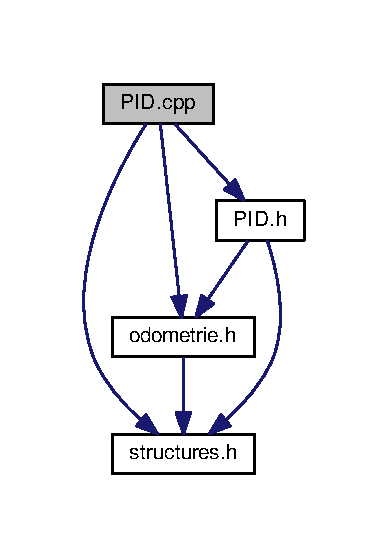
\includegraphics[width=186pt]{_p_i_d_8cpp__incl}
\end{center}
\end{figure}


\subsection{Detailed Description}
Code Proportionnel Intégrateur Dérivateur (\hyperlink{class_p_i_d}{P\+ID}) du grand Robot. Permet de corriger la consigne de sortie en fonction de la consigne d\textquotesingle{}entrée (éviter les oscilations de position et d\textquotesingle{}angle) 

Codé pour \char`\"{}\+Spark core\char`\"{} www.\+spark.\+io

Par \+: Thibaut L\+O\+C\+Q\+U\+ET Octobre 2012 Modification\+: Clément L\+E\+T\+E\+L\+L\+I\+ER Mars 2014 Modification\+: Nicolas S\+O\+B\+C\+Z\+AK Octobre 2016 